\chapter{Core}
	\section{Organisation des packages}

		L'organisation des packages se déroule comme suit :

		\begin{figure}[H]
			\centering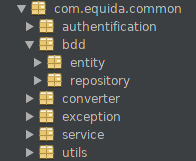
\includegraphics[width=0.33\textwidth, keepaspectratio]{res/package.png}
			\caption{Packages de Core}
		\end{figure}

		\begin{description}
			\item[authentification]{Contient toutes le classes relatives à l'authentification}
			\item[bdd]{Contient toutes les classes relative à la \bdd{}}

			\begin{description}
				\item[entity]{Contient toutes les classes Métiers}
				\item[repository]{Contient toutes les classes qui héritent de CrudRepository}
			\end{description}

			\item[converter]{Contient toutes les classes qui héritent de AttributeConverter}
			\item[exception]{Contient toutes les Exceptions}
			\item[service]{Contient toutes les classes Services}
			\item[utils]{Contient quelques classes utiles (Sha256PasswordEncoder, DateUtils, ...)}
		\end{description}

	\section{Exemple d'Entity}
		%TODO Léa : Parler de comment fonctionnent nos entités, comment ils sont fait et donner un exemple

	\section{Exemple de Repository}
		%TODO Léa : Parler de comment fonctionnent les répository, comment ils sont fait et donner un exemple

	\section{Exemple de Service}
		%TODO Léa : Parler de comment fonctionnent nos Services, comment ils sont fait et donner un exemple

	\section{Exemple d'exception (NotFoundException)}
		Le module Core permet de fournir certaines exceptions. Actuellement elles sont au nombre de 4.

		\begin{figure}[H]
			\centering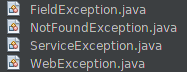
\includegraphics[width=0.30\textwidth, keepaspectratio]{res/exceptions.png}
			\caption{Les différentes exceptions}
		\end{figure}

		\begin{description}
			\item[FieldException]{Permet de signaler une erreur sur un champs d'un formulaire alors que l'information saisie est valide d'un point de vue HTML. On peut par exemple citer un sire qui n'existe pas dans la \bdd{}, un login qui existe déjà, ...}
			\item[NotFoundException]{Permet, notamment, de signaler que l'enregistrement demandé n'existe pas dans la \bdd{} ou bien que l'utilisateur n'est pas autorisé à le voir, comme c'est le cas avec un cheval qui appartient à un autre client par exemple.}
			\item[ServiceException]{Permet de signaler une erreur dans le comportement du Service. Elles sont surtout utilisés pour signaler qu'un champs requis vaut null.}
			\item[WebException]{Permet d'encapsuler une exception pour ne pas gêner l'affichage utilisateur. Lors d'un ServiceException, par exemple, l'envoie d'un WebException permet d'afficher une page d'erreur personnalisée.}
		\end{description}

		Le code des exceptions est plutot simple et court. Voici, par exemple, le code pour NotFoundException.

		\begin{figure}[H]
			\centering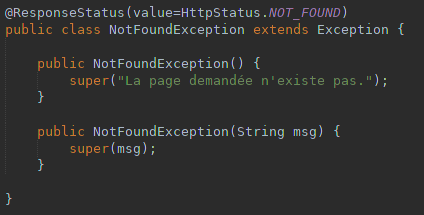
\includegraphics[width=0.75\textwidth, keepaspectratio]{res/NotFoundException.png}
			\caption{Code de NotFoundException}
		\end{figure}

		On y définit un simple message d'erreur et on change le code de réponse HTTP, grace à l'annotation ResponseStatus, pour qu'il envoie le code 404 et affiche la page adéquate.

	\section{Authentification}
		\label{sec:core_authentification}

		Ce package permet de gérer les différentes classes communes à l'authentification de l'utilisateur pour ce qui est du module Rest et WebApp. On y retrouve 2 classes :

		\begin{description}
		   \item[AuthentificationService]{Cette classe implémente l'interface "UserDetailsService". Elle permet pour un login donné d'aller récupérer l'utilisateur correspondant dans la \bdd{} et retourne un objet de type "AuthentificatedUser".}
		   \item[AuthentificatedUser]{Représente l'utilisateur actuellement connecté. Cette classe implémente l'interface "UserDetails". On y retient notamment la classe Compte qui est la classe métier de la table "COMPTE" dans la \bdd{}. Grace à cet attribut on pourra facilement obtenir les informations sur l'utilisateur connecté, par le biais de la méthode "Utilisateur getUtilisteur()".}
	   \end{description}

	   L'authentification sera alors géré de manière différente selon le module. Dans le cas du module WebApp il s'agira d'une connexion par le biais d'une page web tandis que pour l'api Rest on utilisera \href{https://fr.wikipedia.org/wiki/Authentification\_HTTP#M%C3%A9thode\_%C2%AB\_Basic\_%C2%BB}{Basic Authentification}.

	\section{Utils}

		\subsection{DateUtils}

			Cette classe permet de gérer certaines fonctionnalités au niveau des dates. On peut par exemple citer la méthode "boolean isBetween(Date, Date, Date)" qui permet de savoir si la dernière Date est comprise entre les 2 premières. Cette classe permet également d'aficher une date fournit en parametre au format "jour/mois/année" grâce à la méhode "String format(Date)"

		\subsection{Sha256PasswordEncoder}
			\label{subsec:Sha256PasswordEncoder}

			Cette classe permet de gérer le hachage des mots de passes. Elle implémente l'interface "PasswordEncoder". Celle ci fournit une méthode publique "String encode(CharSequence)" retournant en String le hachage, en sha256 dans notre cas, de la chaine de caractère fournit en paramètre. Cette classe est fournit à Spring Security afin de vérifier les informations saisies par l'utilisateur lors d'une connexion. Elle est également utilisé manuellement lors de l'enregistrement d'un nouveau client.
